\documentclass{article}

\usepackage[toc,page]{appendix}
\usepackage{graphicx}
\usepackage{wrapfig}
\usepackage{xcolor}
\usepackage{amsmath}
\usepackage{verbatim}
\usepackage{makeidx}
\usepackage{float}
\usepackage{subfig}
\usepackage[left=1in,top=1in,right=1in]{geometry}

\makeindex

\begin{document}

\begin{center}
\vspace{2cm}
{\Huge\sf\bf RoboSim User's Guide} \\
\vspace{2.5cm}
\begin{center}
	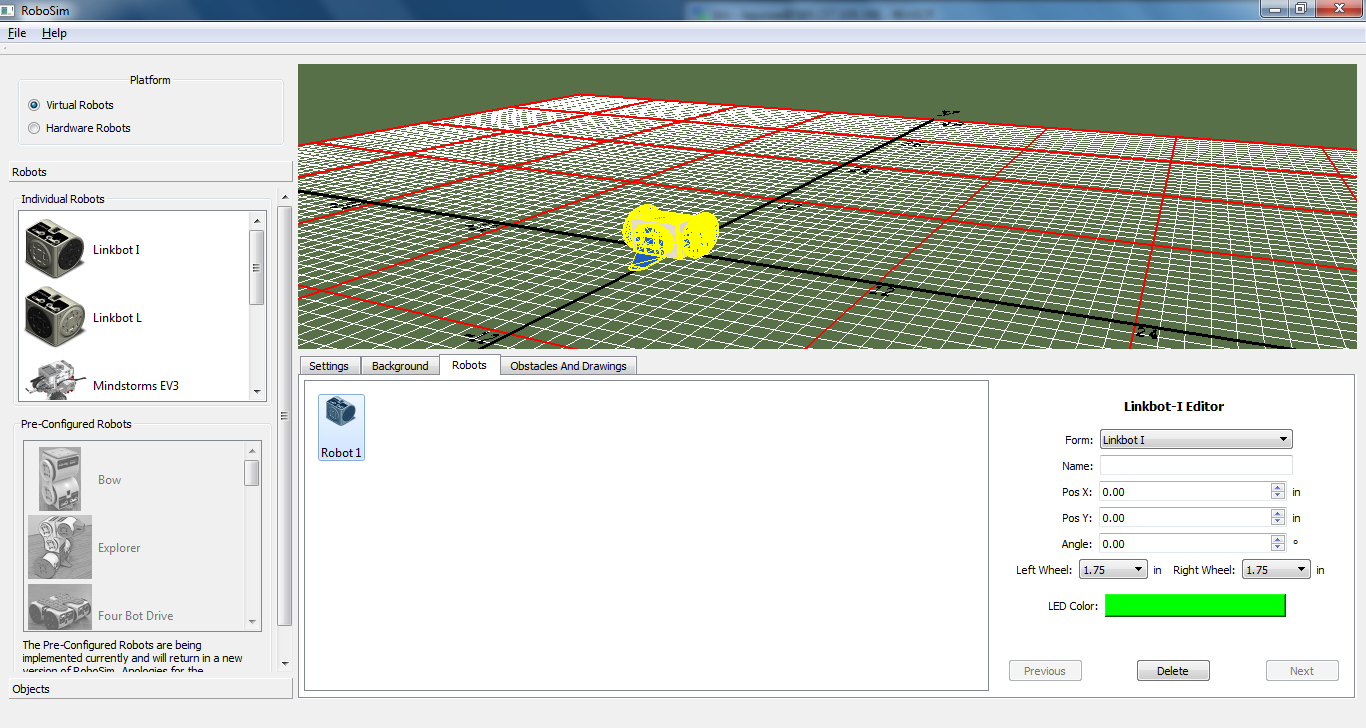
\includegraphics[width=6in]{pictures/gui}
\end{center}
\vspace{1.5cm}
{\Large\bf Version 1.9.90} \\
\vspace{6cm}
Copyright \copyright\ \today\ by UC Davis C-STEM Center, All rights reserved.
\end{center}

\newpage
\tableofcontents
\newpage

%%%%%
%
% Introduction
%
%%%%%
\section{Introduction}
\texttt{RoboSim} is a robot simulation environment, developed by the UC Davis
Center for Integrated Computing and STEM Education (C-STEM) {\color{blue} \bf
(http://c-stem.ucdavis.edu)}, for programming the Barobo Linkbot and LEGO
Mindstorms EV3 and NXT robots.  The same Ch program  can control hardware robots
or virtual robots in RoboSim without any modification.

%%%%%
%
% The GUI
%
%%%%%
\section{RoboSim GUI}
\label{sec:gui}
RoboSim can be conveniently launched by double clicking its icon

\includegraphics[height=24pt]{pictures/robosim} on the desktop.  The RoboSim
graphical user interface (GUI), shown in Figure \ref{fig:gui}, allows the user
to change between hardware and virtual robots when a Ch robot program is
executed.  There is no save button within the GUI, all changes made are
automatically saved.  The RoboSim GUI is the place to configure the RoboSim
Scene for interacting with the virtual robots.  It is designed to be easy to use
fro configuring the Scene and the robots within it.  There are four pieces of
the GUI that hold four separate configurations.
\begin{itemize}
	\item Platform Selection
	\item Add To Scene Selection
	\item Scene View
	\item Scene Configuration
\end{itemize}

\begin{figure}[H]
	\begin{center}
		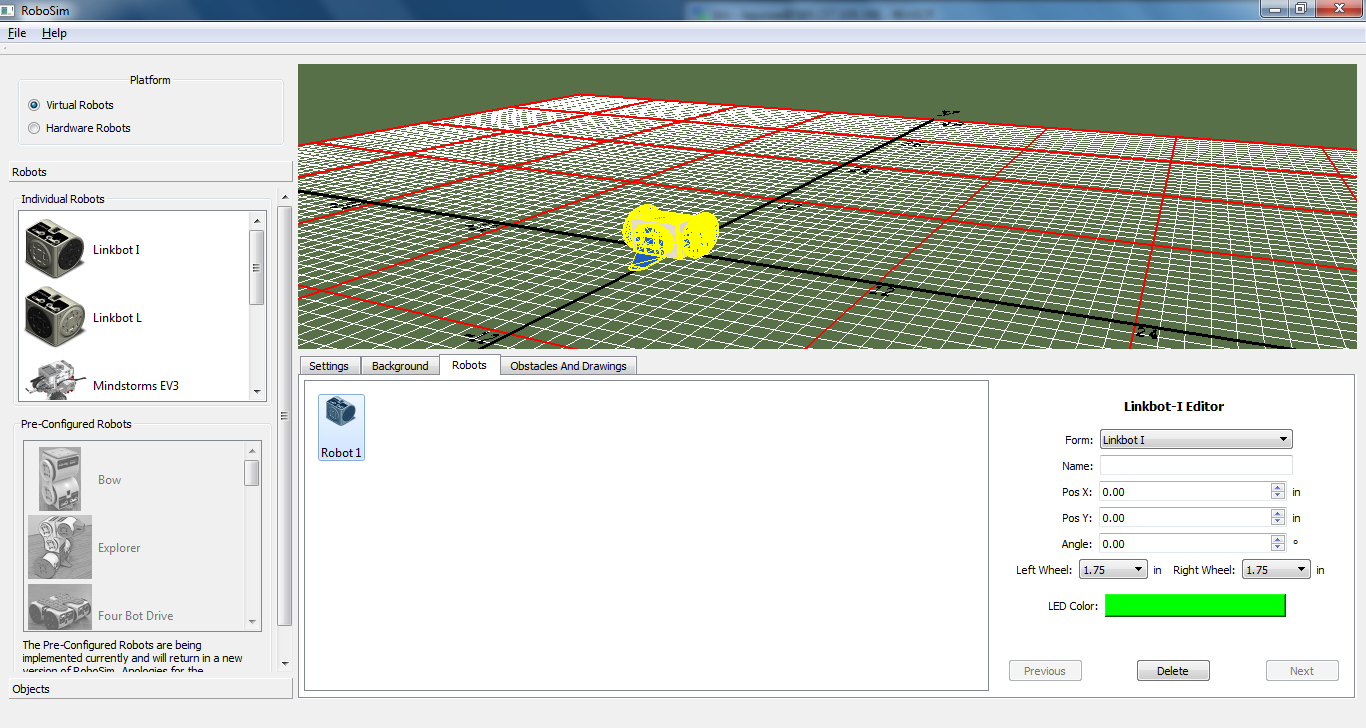
\includegraphics[width=5in]{pictures/gui}
	\end{center}
	\caption{The RoboSim GUI.}
	\label{fig:gui}
\end{figure}

\subsection{Platform Selection}
The {\bf Platform} entry as shown in Figure \ref{fig:platform}, allows the user
to decide whether a Ch program controls the hardware or virtual robots.  Each
time a new Ch program is started, it will check the setup based on this entry.
For a Ch robot program to control a virtual robot, check the box for {\bf
Virtual Robots}.  If the box for {\bf Hardware Robots} is checked, a Ch
program will control the physical hardware robots.
\begin{figure}[H]
	\begin{center}
		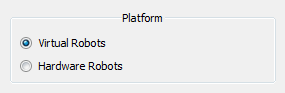
\includegraphics[width=3in]{pictures/gui_platform}
	\end{center}
	\caption{Initial robot configuration dialog.}
	\label{fig:platform}
\end{figure}

\subsection{Add To Scene Selection}
The accordion along the left hand side holds all of the elements which can be
added into the scene as shown in Figure \ref{fig:add}.
\begin{figure}[H]
	\begin{center}
		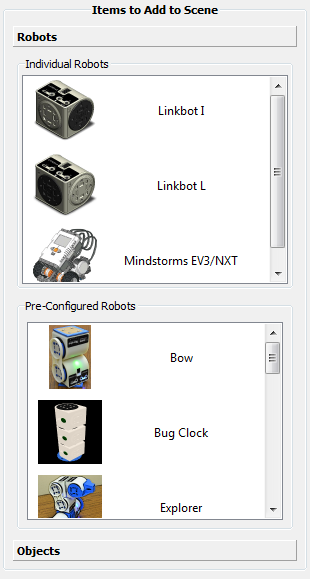
\includegraphics[width=3in]{pictures/gui_add}
	\end{center}
	\caption{Add To Scene: selection of items to add to Scene.}
	\label{fig:add}
\end{figure}
There are two groups: Robots and Obstacles and Drawings.  The robots group has
the list of robots available to be added into the scene which includes the
Linkbot-I, Linkbot-L, Mindstorms EV3, and Mindstorms NXT.  The Obstacles and
Drawings group holds the extra elements  for the scene.  The difference between
obstacles and drawings can be summarized as follows:
\begin{itemize}
	\item Obstacles have mass and interact with the robots
	\item Drawings do not have mass and are only drawn on the screen
\end{itemize}

The possible obstacles are Box, Cylinder, and Sphere.  The drawings are Lines,
Points, and Text.  To add a desired object to the scene, click and drag it onto
the proper tab of the Scene Configuration.  A drop indicator will show up when
the object can be added as shown in Figure \ref{fig:drop}.  Once the object has
been added, it will show up in the Scene View.
\begin{figure}[H]
	\begin{center}
		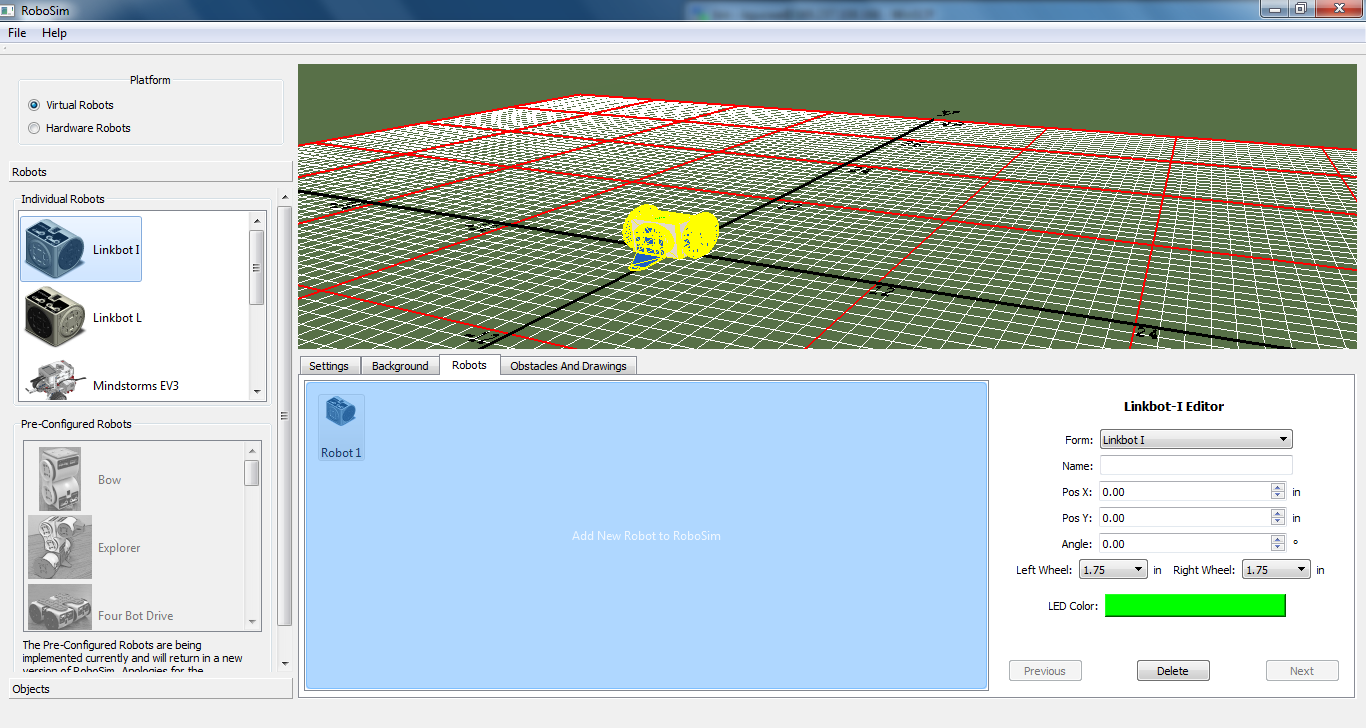
\includegraphics[width=5in]{pictures/gui_drop}
	\end{center}
	\caption{Drop Indicator for adding a robot.}
	\label{fig:drop}
\end{figure}

\subsection{Scene View}
The Scene View is a live version of the RoboSim Scene which shows the current
state of the configuration.  All keyboard and mouse interactions work as
expected from the RoboSim Scene.  Clicking a robot or obstacle selects it in
yellow and makes it the current one in the Scene Configuration section to be
able to edit its properties.  As elements of the scene are changed, their state
is automatically updated in the Scene View.  Once ready to run code, the student
starts the code and the RoboSim Scene will pop up showing the same state as
shown in the GUI.

Since there are no limits placed on how items can be positioned in the Scene,
it is a possibility that two or more can be configured to be overlapping.  When
this happens, all objects which overlap will be highlighted in red in the scene
view and a message will appear for the user stating 'Objects are colliding'.
To fix the problem, move one or more of the objects away from the others.  As
soon as RoboSim detects there is no longer an intersection, the message will
disappear and the red highlighting will disappear.

\subsection{Scene Configuration}
The main section of the GUI is the Scene Configuration tab bar.  Each tab
holds one piece of the configuration parameters for the Scene.

\subsubsection{General Configuration}
The first one is the general configuration options.  The parameters listed here
affect the whole scene by changing how it looks and behaves.

\paragraph{Units}
Simulations within RoboSim can be run either in {\bf US Customary} units
consisting of inches, degrees, and seconds or {\bf Metric} units with
centimeters, degrees, and seconds.  Changing units will effect the grid spacing
drawn beneath the robots and the spacing between robots.  Changing between these
two options will change the labels within the GUI to indicate the units being
used.

\paragraph{Tracing}
{\bf Tracing} where robots have been can be enabled by selecting the check box
'Enable Robot Position Tracing', as shown in Figure \ref{fig:gui}.  When the
tracing is enabled, lines following the robot trajectories will be drawn for
each robot.  Mobot tracking lines will be in a green color and Linkbot tracking
lines will be in the color matching the Linkbot LED.

\paragraph{Grid Configuration}
To be able to see how far robots have moved, a grid is enabled under the robots.
There are six options to alter the layout of the grid lines under the {\bf Grid
Configuration}.  The minimum and maximum extends of the grid for both the X and
Y directions can be specified individually.  Rectangular grids of any size can
be created in any of the quadrants.  Hashmarks are the red lines drawn within
the configuration images.  By default, the distance between two hashmarks is 12
inches in US Customary units and 50 centimeters in Metric units.  Tics are the
most frequent lines drawn in a light gray.  By default, the distance between two
tics is 1 inch in US Customary units and 5 centimeters in Metric units.

Switching between US Customary and Metric units will change these default values
to logical starting points for the metric system.  The 'Reset to Defaults'
button will allow the default values for both US Customary and Metric to be
reinstated after they have been changed.  Depending upon which units are
currently selected, either the US Customary defaults, shown in Figure
\ref{fig:grid_us}, or the Metric defaults, as shown in Figure
\ref{fig:grid_metric}, will be set.
\begin{figure}[H]
	\begin{center}
		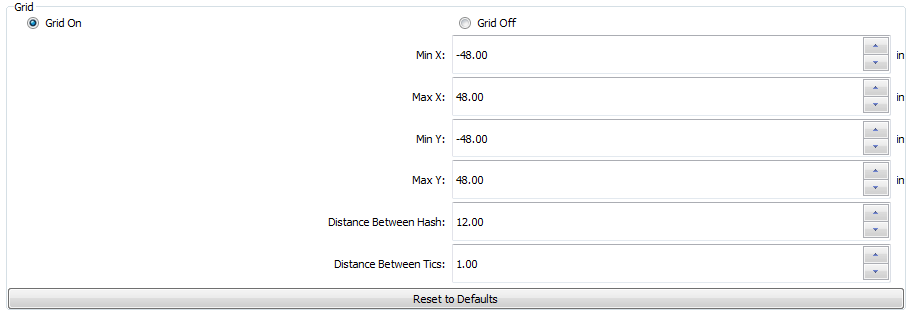
\includegraphics[width=4in]{pictures/gui_grid_us}
	\end{center}
	\caption{Default US Customary Grid Spacing.}
	\label{fig:grid_us}
\end{figure}
\begin{figure}[H]
	\begin{center}
		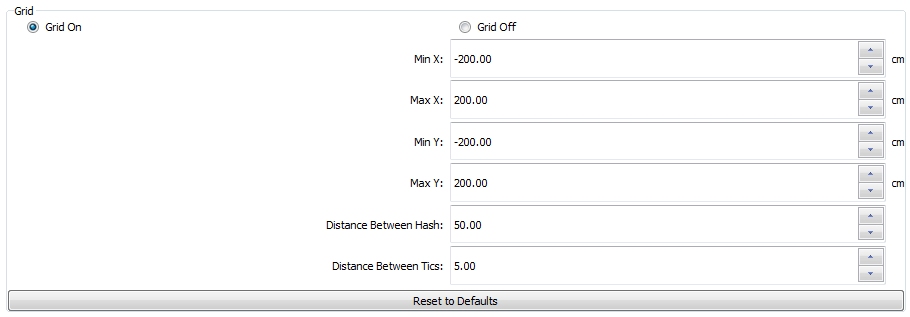
\includegraphics[width=4in]{pictures/gui_grid_si}
	\end{center}
	\caption{Default Metric Grid Spacing.}
	\label{fig:grid_metric}
\end{figure}

\subsubsection{Background}
The background behind the robots can be changed to display different views for
the Scene.  There are four default options for the robots.  Users can write
their own and add them to the list if desired.  Details on how to write a
RoboSim Background are detailed in Appendix \ref{app:backgrounds}.  The default
backgrounds are None, RoboPlay 2014, RoboPlay 2015, RoboPlay 2016, RoboPlay
2017, Barobo activity mat, and Outdoors.  The 'None' background is a completely
black scene with the robots moving through the empty space.  The challenge
boards from the 2014, 2015, 2016, and 2017 RoboPlay Challenge Competitions are
included to easily play on the mats.  The borders are solid obstacles so that
the robots are not able to run off the sides.  The 'Outdoors' background is the
original RoboSim Scene consisting of the green grass and blue sky.  Selecting
each one automatically changes the background in the Scene View.

\paragraph{Adding Custom Backgrounds}
Users are able to create and add custom backgrounds to RoboSim through the 'Add
New Background Folder' button in the lower right corner.  By clicking the button
and selecting a folder, RoboSim will look through each subfolder to see if it is
a valid RoboSim Background file to add and display in the list in addition to
the default ones available already.  Each time RoboSim launches it looks through
this folder to find any new Background files which have been created.

Creating custom backgrounds can be done by users and shared with others.
Appendix \ref{app:backgrounds} explains how to make the files necessary for
RoboSim to load the background information.

\subsubsection{Robots}
All  of the robots in the Scene are configured here.  The Robot List
(see Figure \ref{fig:robot_list}) holds all of the robots currently in the
Scene.  Robots are dragged from the 'Add To Scene' Selection List to this
location to be included in the Scene.
\begin{figure}[H]
	\begin{center}
		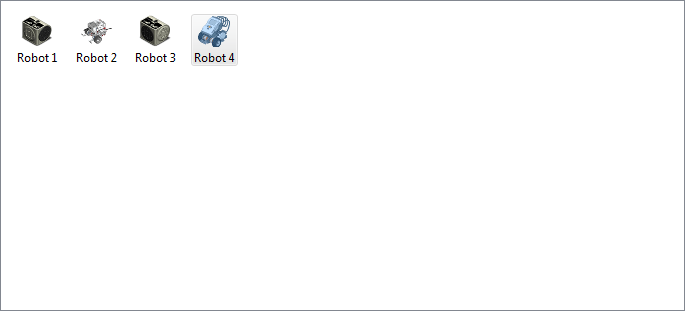
\includegraphics[width=3in]{pictures/gui_robot_list}
	\end{center}
	\caption{Robot List: all robots in the Scene.}
	\label{fig:robot_list}
\end{figure}
Clicking on one of the robots makes it the current one which means two things:
it is highlighted yellow in the Scene View and the robot editor to the right is
filled with the information about this robot.  To the right is the Robot Editor
dialog.  All information about a robot that can be changed is done here.  The
possible options change depending upon the selected robot.  Figure
\ref{fig:editorI} shows the dialog for a Linkbot-I as an example.
\begin{figure}[H]
	\begin{center}
		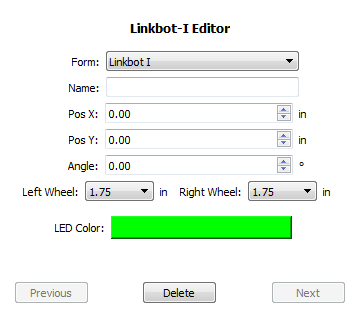
\includegraphics[width=3in]{pictures/gui_editorI}
	\end{center}
	\caption{Robot Editor: editor for a Linkbot-I.}
	\label{fig:editorI}
\end{figure}
The dropdown allows the user to change the type of robot which in turn changes
the options.  A name for the robot can be entered if desired.  The X and Y
positions of the robot can be changed either through the arrows or typing in a
desired number.  The robot angle is measured from the X-axis rotating in a
counter-clockwise direction.  Left and right wheels can be added separately to
the robot.  The options are all of the sizes of wheels made for the Linkbots.
Wheel size options for the Mindstorms robots are the two which are distributed
with the robot (1.1 and 1.6 inch radii).  The LED color button brings up a color
picker dialog to select any desired color.  The buttons at the bottom remain the
same for each robot.  The Previous and Next buttons allow the previous or next
robot in the list to become the one selected for editing.  The Delete button
deletes the robot from the Scene.

\subsection{Preconfigured Robot Configurations}
In addition to positioning robots independently within the RoboSim, some {\bf
Preconfigured Robot Configurations}, as shown in Figure \ref{fig:preconfig},
which represent commonly used Linkbot configurations  are available to the user.
Selecting one of these options will display a picture of the configuration built
with the hardware Linkbots and corresponding to a Ch robot program presented in
Chapter $13$ in the book {\em Learning Robot Programming with Linkbot for the
Absolute Beginner}.  When one of these options is selected, the specific
configuration for this setup is passed into Ch and robots specified in the
individual robot configuration are ignored.  To switch back to the individual
configuration, just unselect the selected preconfigured robot configuration.
\begin{figure}[H]
	\begin{center}
		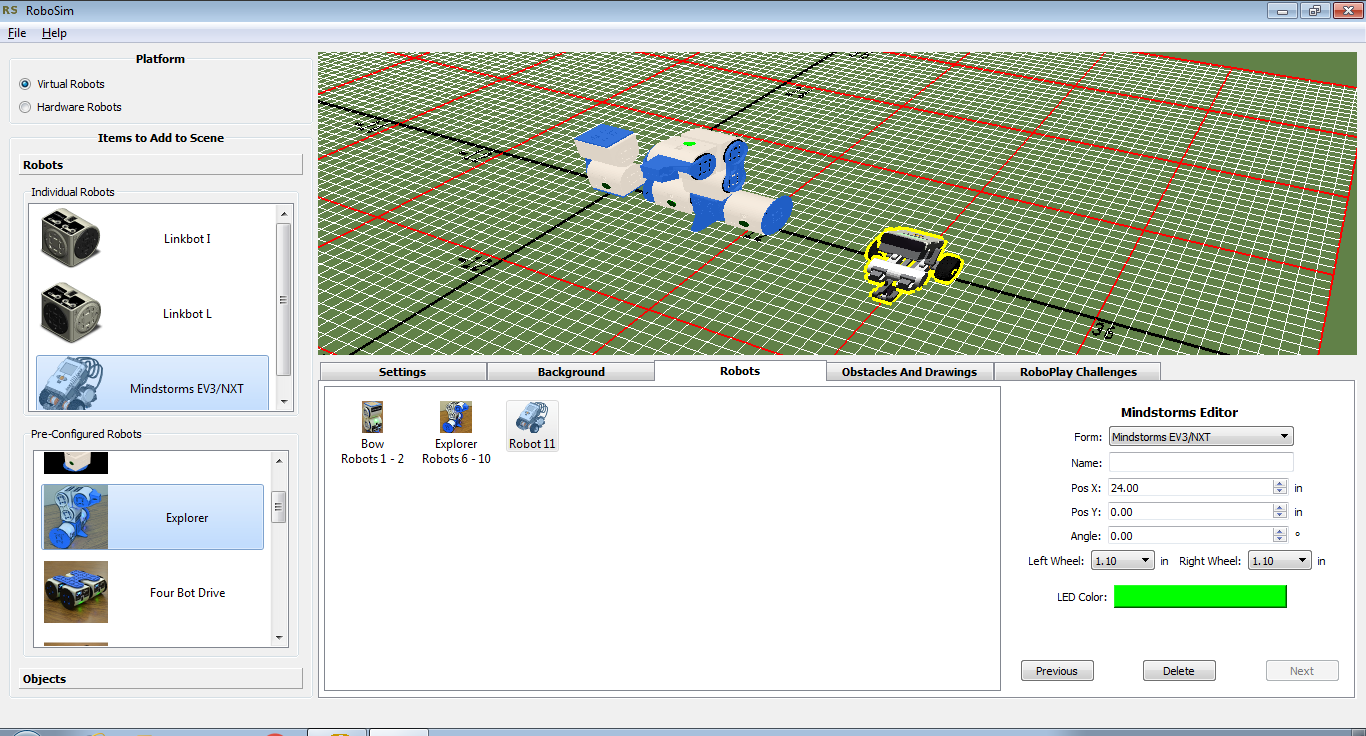
\includegraphics[width=6in]{pictures/gui_preconfig}
	\end{center}
	\caption{Preconfigured Linkbots.}
	\label{fig:preconfig}
\end{figure}

\subsubsection{Obstacles and Drawings}
The obstacles and drawings tab is organized in an identical manner to the Robots
tab.  A list of the objects in the scene are on the left.  New ones are dragged
from the left of the GUI into this list.  An editor for each object is on the
right.  The information in the editor has a few general sections which change
slightly depending upon the specific item being edited.  The physical properties
of the object, such as the length, width, and height of a box or the radius of
the sphere, the object's position in space in X, Y, and Z directions, mass of
the object, and the color.  A few obstacles which were created for the RoboPlay
Challenge Competitions are included as well as generic blocks and spheres.
\begin{figure}[H]
	\begin{center}
		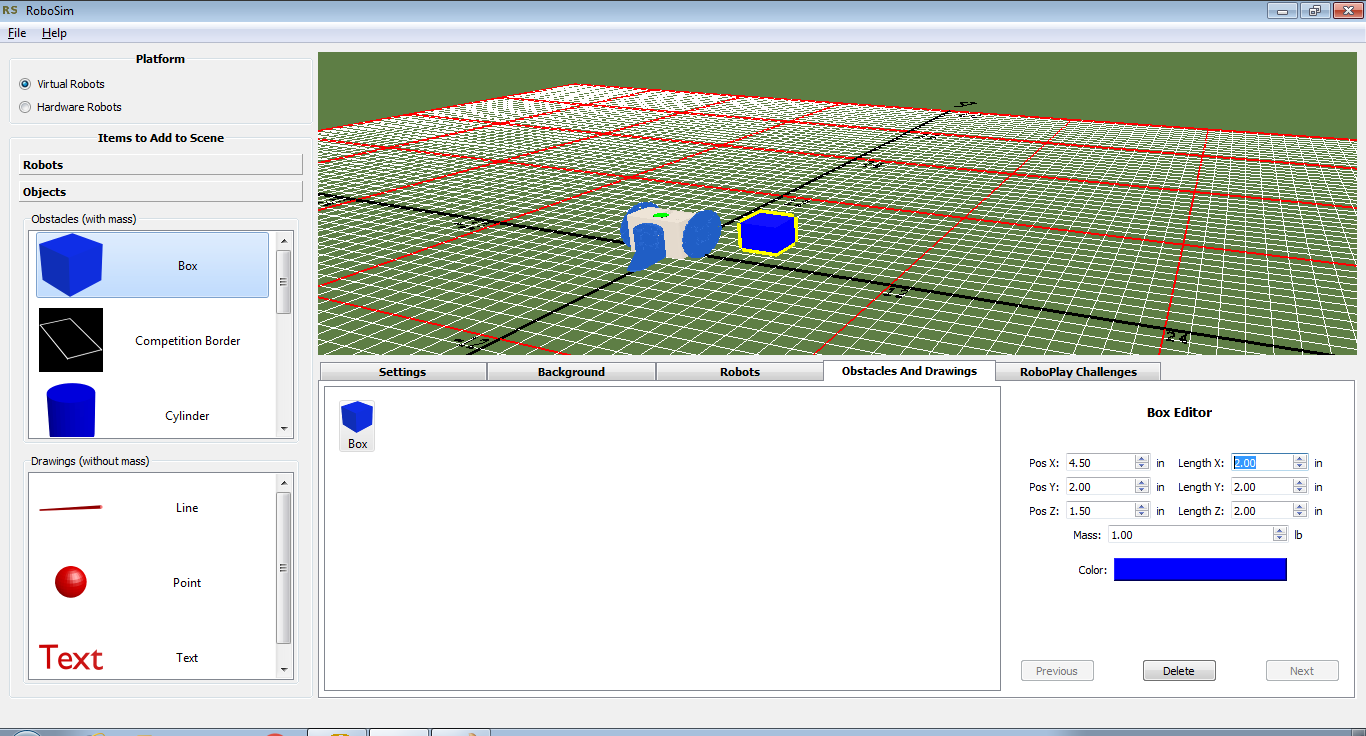
\includegraphics[width=6in]{pictures/gui_obstacles}
	\end{center}
	\caption{Linkbot with a Box obstacle.}
	\label{fig:obstacle}
\end{figure}

\subsubsection{RoboPlay Challenges}
All Challenges from the 2014-2017 RoboPlay Challenge Competitions which can be
completed within RoboSim are included in a separate tab.  These challenges load
up the Challenge Background, and all of the appropriate robots and obstacles to
complete the challenge as outlined in the challenge booklets.
\begin{figure}[H]
	\begin{center}
		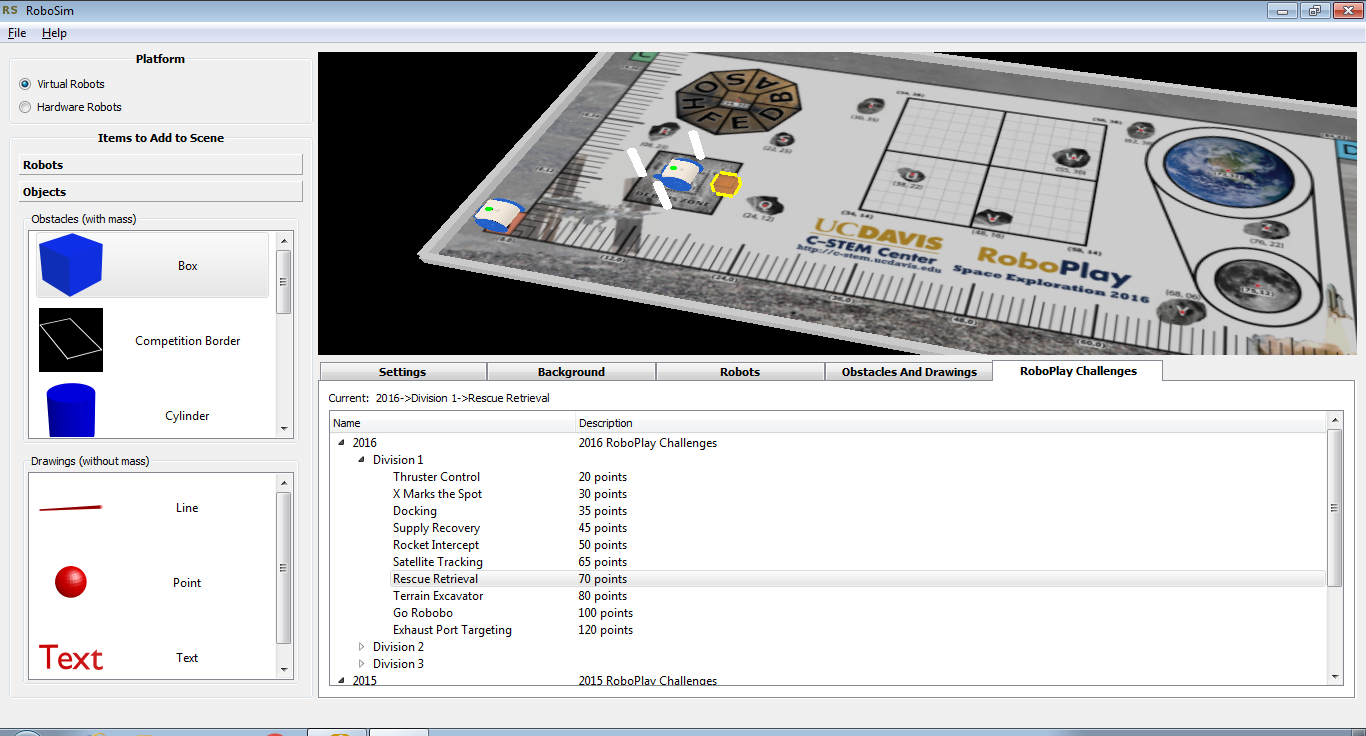
\includegraphics[width=6in]{pictures/gui_challenges}
	\end{center}
	\caption{Challenge List.}
	\label{fig:challenges}
\end{figure}

%%%%%
%
% GUI Cheat Sheet
%
%%%%%
\section{Interacting with the GUI: Cheat Sheet}
\subsection{Adding a Robot}
The list of robots which can be added to the Scene are under the robots group
of the 'Add To Scene' accordion as shown in Figure \ref{fig:add}.  The list of
robots in the scene is in the Robots tab of the Scene Configuration.  Click and
drag a robot from the left to the right and drop it onto the list.  This add it
into the Scene.  The robot should now be in the Robot List as well as drawn in
the Scene View.

\subsection{Deleting a Robot}
To delete a robot already in the Scene, it first has to be selected to become
the current robot.  This is shown in two ways: it is highlighted yellow in the
Scene View and is selected blue in the Robot List.  To select a robot, it can
be clicked in either of these locations.  Deleting can be accomplished by
either pressing the delete key on the keyboard or the delete button in the
robot editor.

\subsection{Editing an Item}
If a robot is selected, its information can be edited.  Selecting can be done
by clicking either the robot in the Scene View to highlight it or in the robot
list.  Once the robot is selected, its information is loaded into the editor to
the right of the Robot List.  Changing any of this information will be
reflected immediately in the Scene View.

\subsection{Colliding Objects}
Since there are no limits placed on how items can be positioned in the Scene,
it is a possibility that two or more can be configured to be overlapping.  When
this happens, all objects which overlap will be highlighted in red in the scene
view and a message will appear for the user stating 'Objects are colliding'.
To fix the problem, move one or more of the objects away from the others.  As
soon as RoboSim detects there is no longer an intersection, the message will
disappear and the red highlighting will disappear.

%%%%%
%
% Running a Ch Program
%
%%%%%
\section{Running a Ch Program with RoboSim}
Once the simulation environment has been configured with the RoboSim GUI in
Section \ref{sec:gui}, the user can run Ch programs in ChIDE to control the
virtual robots.  The RoboSim GUI should remain open while simulating robots.
Once it is closed, the system will revert to hardware mode.  The RoboSim scene
with virtual robots for each simulation are created upon running a Ch program.
For example, when the Ch program {\tt moveforward3.ch} below
\begin{verbatim}
/* File: moveforward3.ch
   Move forward for Linkbot-I as a two-wheel vehicle */
#include <linkbot.h>
CLinkbotI robot;

/* connect to the paired robot and move to the zero position */
robot.connect();
robot.resetToZero();

/* move forward by rolling two wheels for 360 degrees */
robot.moveForward(360);
\end{verbatim}
\noindent
is executed in ChIDE, a RoboSim scene shown in Figure \ref{fig:robosim_scene}
will be displayed.
\begin{verbatim}
    Paused: Press any key to start
\end{verbatim}
is displayed in the RoboSim scene to reminder the user that the virtual robot
will not move until the user presses any key on the keyboard. This gives the
user an opportunity to examine the RoboSim scene before the motion begins.
\begin{figure}[H]
	\begin{center}
		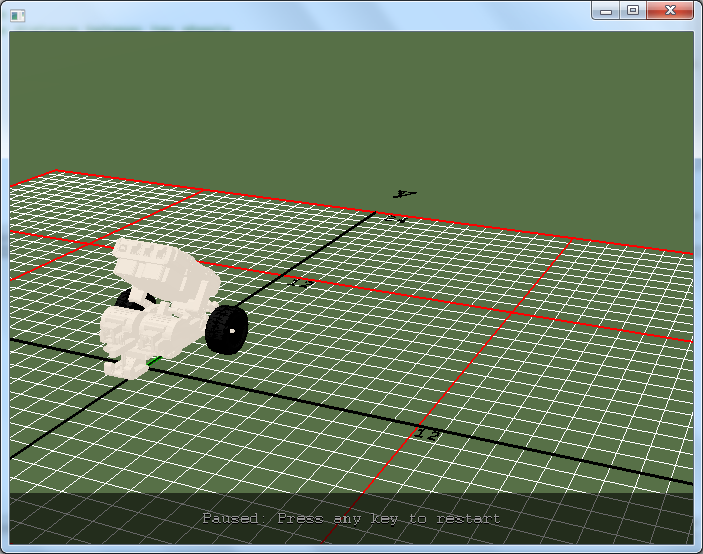
\includegraphics[width=3in]{pictures/robosim_scene}
	\end{center}
	\caption{A RoboSim scene with a virtual robot at its starting position.}
	\label{fig:robosim_scene}
\end{figure}

While a robot is moving in the RoboSim scene, the user can press any key to
pause the motion of the robot.  When the motion is paused, the message
\begin{verbatim}
    Paused: Press any key to restart
\end{verbatim}
will be displayed in the RoboSim scene. The user can press any key to restart
the motion.

When the user presses the 't' key, the robot trajectory is tracked in a green
line in the RoboSim scene as shown in Figure \ref{fig:robosim_tracked}.
\begin{figure}[H]
	\begin{center}
		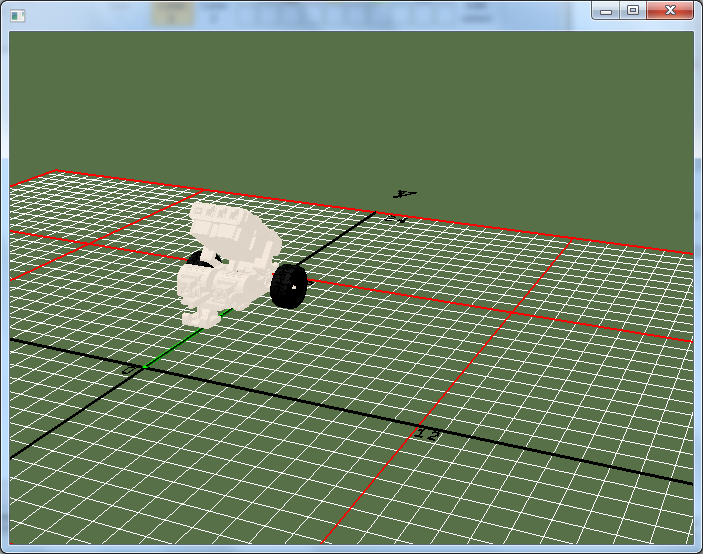
\includegraphics[width=3in]{pictures/robosim_tracked}
	\end{center}
	\caption{A RoboSim scene with a virtual robot and its trajectory tracked.}
	\label{fig:robosim_tracked}
\end{figure}

When the program is finished, the message
\begin{verbatim}
    Paused: Press any key to end
\end{verbatim}
will be displayed in the RoboSim scene.  Pressing any key, the RoboSim scene
will disappear.

%%%%%
%
% Interacting with RoboSim Scene
%
%%%%%
\section{Interacting with a RoboSim Scene}
The user can interact with a RoboSim scene through the keyboard and mouse.

The ground plane is for reference only.  It is designed to disappear when
viewing the robots from below to be able to inspect the movement from all
angles.

\subsection{Keyboard Input}
The RoboSim scene responds to keyboard input as outlined in Table
\ref{tab:keys}.  As described in the previous sections, the 't' key will toggle
the tracking of robot trajectories.

\begin{table}[H]
	\begin{center}
	\begin{tabular}{c | l }
		\hline \hline
		\textbf{key} & \textbf{action} \\ \hline
		1 & return to home camera position \\
		2 & set camera to overhead view \\
		C & center the current robot in the View (GUI only) \\
		N & toggle grid line numbering \\
		R & toggle robot visibility and enable tracking \\
		T & toggle robot tracking \\
		any other key & Pause and resume the simulation \\
		\hline \hline
	\end{tabular}
	\caption{Keyboard input for RoboSim}
	\label{tab:keys}
	\end{center}
\end{table}

There are two views available to the user.  The default view, which can be
toggled with the '1' key, is from behind the robots looking into the second
quadrant.  This view can be seen in any of the RoboSim scene screenshots within
this document, except for Figure \ref{fig:robosim_overhead} which shows the
overhead view.  The '2' key moves the camera directly above the origin looking
down on the scene creating a 2D viewpoint of the robots.
\begin{figure}[H]
	\begin{center}
		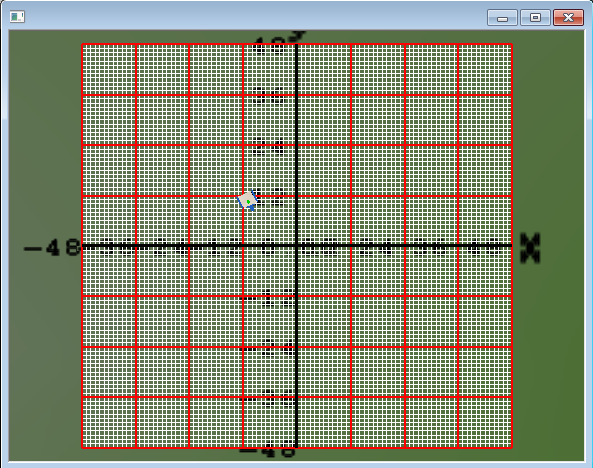
\includegraphics[width=3in]{pictures/robosim_overhead}
	\end{center}
	\caption{A RoboSim scene with the overhead viewing angle.}
	\label{fig:robosim_overhead}
\end{figure}

In the RoboSim GUI the highlighted robot is the one which is being edited
currently.  To center this robot in the Scene View, press the 'c' key.  This
will move the camera to put this robot at the center of the view.

The 'n' key allows the user to toggle the display of the grid numbering.  X and
Y numbering is by default enabled and given for every hashmark on the grid.

The 'r' key will toggle the display of virtual robots or robot trajectories.  It
will also disable collision checking between robots so that trajectories can be
intersecting.  This feature is useful when the user would like to view a
trajectory traced by a robot without the virtual root blocking the trajectory.
Figure \ref{fig:robosim_norobot} shows a RoboSim scene with a tracked robot
trajectory only.
\begin{figure}[H]
	\begin{center}
		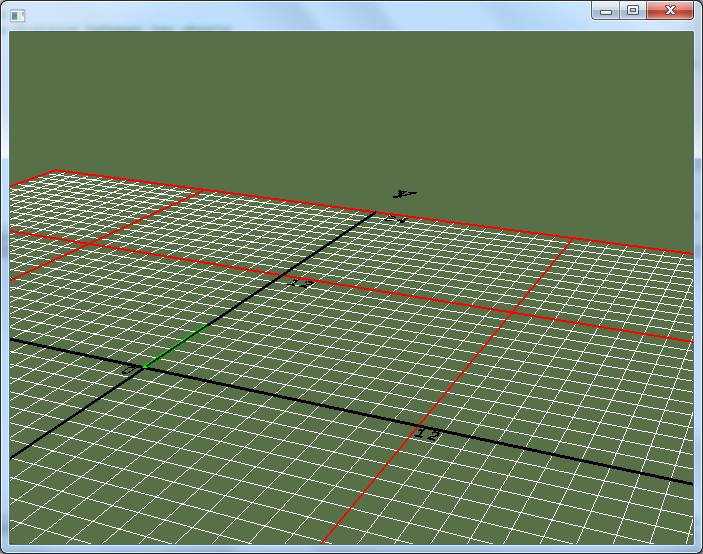
\includegraphics[width=3in]{pictures/robosim_norobot}
	\end{center}
	\caption{A RoboSim scene with a tracked robot trajectory only.}
	\label{fig:robosim_norobot}
\end{figure}

As described in the previous section, the motion of robots in the RoboSim scene
can be paused and restarted by pressing any other key on the keyboard.

\subsection{Mouse Input}
Clicking on a robot in a RoboSim scene will enable a pop up which displays the
robot's name, if set in the RoboSim GUI, the robot number, and the current
position of the robot, as shown in Figure \ref{fig:robosim_pos}.  Clicking again
the displayed position for the robot will disappear.
\begin{figure}[H]
	\begin{center}
		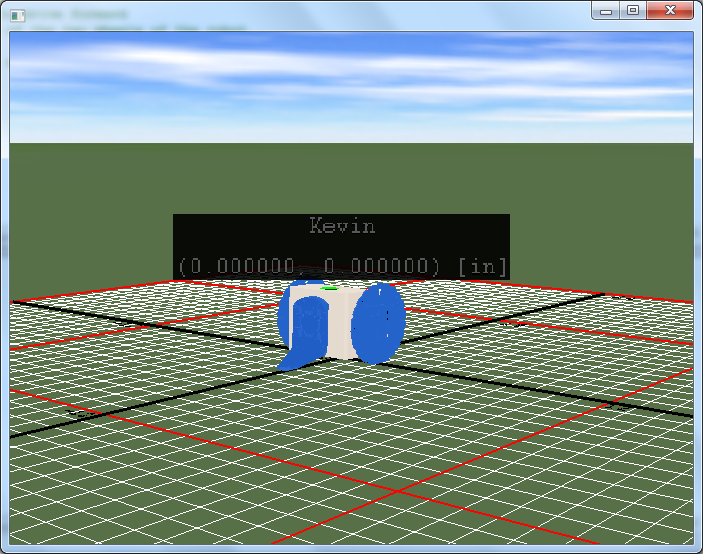
\includegraphics[width=3in]{pictures/robosim_pos}
	\end{center}
	\caption{A RoboSim scene with a virtual robot and its position displayed.}
	\label{fig:robosim_pos}
\end{figure}

The user can execute a Ch robot program in debug mode in ChIDE, line by line,
with the command {\tt Next}. At the end of each motion statement, the user can
click the robot in the RoboSim scene to obtain the X and Y coordinates of the
robot.  The ability to obtain the X and Y coordinates of a robot during its
motion along a trajectory can be very useful for learning many math concepts.

The mouse can be used to move the camera around the scene.  Holding the left
mouse button and dragging the mouse pans the camera as outlined in Table
\ref{tab:buttons}.  Holding the right mouse button and dragging the mouse
enables scaling of the view by zooming in and out.  Holding both left and right
mouse buttons and dragging changes the location of the camera within the scene.

The ground plane is for reference only.  The ground plane will disappear when
viewing the robots from below so that the user can inspect the movement from all
angles.

\begin{table}[H]
	\begin{center}
	\begin{tabular}{c | l }
		\hline \hline
		\textbf{button} & \textbf{action} \\ \hline
		Hold left mouse button and drag& rotate camera \\
		Hold right mouse button and drag& zoom in and out \\
		Hold both left and right buttons,  and drag & pan around scene \\
		Click on a robot & display the robot position\\
		\hline \hline
	\end{tabular}
	\caption{Mouse input for the RoboSim scene.}
	\label{tab:buttons}
	\end{center}
\end{table}

%%%%%
%
% Differences between Virtual and Hardware
%
%%%%%
\section{Differences Between Virtual and Hardware Robots}
RoboSim has some different options which affect the performance of the
simulation.  These are options which are passed into the constructor of the
robots that are not available within hardware.  The RoboSim GUI writes all of
the options into a user configuration file that has to be changed each time a
new code is to be run.  However, users can manually write configuration files
specific to each code.  To tell RoboSim to use a custom configuration file over
the global one, pass the name of the file into the first robot constructor call
in the file.  RoboSim will look in the same folder to find the configuration
file, if it is not found, then it will use the default one.
\begin{verbatim}
#include <linkbot.h>
CLinkbotI robot("testrc");
\end{verbatim}

%%%%%
%
% APPENDIX
%
%%%%%
\newpage
\appendix
\section{Appendix: Manual Configuration File Generation}
\label{app:xml}
All options available in the RoboSim GUI can be done manually as well as adding
in more advanced features which are not necessary to be exposed to all users in
the GUI.  There are four sections to the configuration file.  The header,
configuration, ground, and simulation sections.  Each holds specific types of
information about the simulation to be run.

\subsection{Header}
The header is one line and specifies to RoboSim that this is a valid xml file.
This line should be placed at the start of each simulation file.
\begin{verbatim}
<?xml version="1.0" encoding="UTF-8"?>
\end{verbatim}

\subsection{Configuration Section}
General parameters about the simulation can be added within the config section.
Each one is its own line placed between the starting \verb%<config>% and ending
\verb%</config>%.
\begin{verbatim}
<config>
</config>
\end{verbatim}

\subsubsection{Version}
\begin{verbatim}
<version>1</version>
\end{verbatim}
The version of the XML configuration file.  Updated internally when new
non-backwards compatible changes are made.

\subsubsection{Grid}
\begin{verbatim}
<grid major="12" tics="1" minx="-48" maxx="48" miny="-48" maxy="48"/>
\end{verbatim}
The grid boxes from the GUI put their information here.   \verb%major% are the
red hashmarks and \verb%tics% are the gray tick marks.  \verb%minx% and
\verb%maxx% are the minimum and maximum distances along the X-axis for the
grids, respectively.  \verb%miny% and \verb%maxy% are the complements for the
Y-axis.

\subsubsection{Units}
\begin{verbatim}
<units>1</units>
\end{verbatim}
\verb%units%: 1 for US Customary and 0 for Metric.

\subsubsection{Trace}
\begin{verbatim}
<trace>1</trace>
\end{verbatim}
Setting to trace robot location with lines on the ground.  1 for on; 0 for off.

\subsubsection{Pause}
\begin{verbatim}
<pause>1</pause>
\end{verbatim}
The simulation can either start paused waiting for a user to press a key to
start or it will start as soon as it is ready.  Passing 0 to this option starts
the simulation; while 1 pauses it at the beginning.

\subsubsection{Real Time}
\begin{verbatim}
<realtime>1</realtime>
\end{verbatim}
The simulation can run faster than real time.  Passing 0 to this option allows
the simulation to run as fast as the computer can simulate it.

\subsubsection{Mu}
\begin{verbatim}
<mu ground="0.9" body="0.3"/>
\end{verbatim}
The coefficient of friction can be altered between the robots and the ground and
between robots themselves.  The default values are given here.

\subsubsection{Coefficient of Restitution}
\begin{verbatim}
<cor ground="0.3" body="0.3"/>
\end{verbatim}
The coefficient of restitution can be altered between the robots and the ground
and between robots themselves.  The default values are given here.  The COR is a
measure of how bouncy a surface is.  Small values correspond to hard surfaces
while larger values are for softer surfaces.

\subsection{Ground Section}
\label{app:xml:obstacles}
The ground section holds the solid bodies which are a part of the ground for
which the robots to interact.  The objects do not need to be on the ground
plane.  They can be floating in space but are still a part of the ground
objects.  Each object has a mass associated with it and interacts in the
simulation.  An object with heavy mass cannot be moved by the robots, while
lighter objects will be pushed around.  Everything to be added is put between
the \verb%<ground>% tags.
\begin{verbatim}
<ground>
</ground>
\end{verbatim}

\subsubsection{Box}
\begin{verbatim}
<box id="0" mass="1">
    <size x="1" y="1" z="1"/>
    <color r="0" g="0" b="1" alpha="1"/>
    <position x="1" y="1" z="1"/>
    <rotation psi="1" theta="1" phi="1"/>
</box>
\end{verbatim}
The ground box is configured with the mass, color, size, position, and rotation
parameters.  Each item has an unique id to identify it within the RoboSim GUI.
Mass is given as the total mass for the object in kilograms.  The size gives the
lengths in the X, Y, and Z directions.  Color defines the RGB colors as well as
the alpha transparency of the box.  An alpha of 1 is opaque; 0 is transparent.
Position gives the X, Y, and Z location of the center of the box.  The rotation
gives the three Euler Angles of the box.

\subsubsection{Cylinder}
\begin{verbatim}
<cylinder id="0" mass="1" axis="1">
    <size radius="1" length="10"/>
    <color r="0" g="0" b="1" alpha="1"/>
    <position x="1" y="1" z="1"/>
    <rotation psi="1" theta="1" phi="1"/>
</cylinder>
\end{verbatim}
The ground cylinder is configured with the mass, axis, color, size, position,
and rotation parameters.  Each item has an unique id to identify it within the
RoboSim GUI.  Mass is the total mass of the object.  Axis is the long axis for
the object given the convention 1=X, 2=Y, and 3=Z.  The size gives the radius
and length of the cylinder.  Color defines the RGB colors as well as the alpha
transparency of the box.  An alpha of 1 is opaque; 0 is transparent.  Position
gives the X, Y, and Z location of the center of the cylinder.  The rotation
gives the three Euler Angles.

\subsubsection{Sphere}
\begin{verbatim}
<sphere id="0" mass="1">
    <size radius="1"/>
    <color r="0" g="0" b="1" alpha="1"/>
    <position x="1" y="1" z="1"/>
</sphere>
\end{verbatim}
The ground sphere is configured with the mass, size, color, and position
parameters.  Each item has an unique id to identify it within the RoboSim GUI.
Mass is the total mass of the object.  The size gives the radius of the sphere.
By default the cylinder is drawn with the long axis along the X-axis.  Color
defines the RGB colors as well as the alpha transparency of the box.  An alpha
of 1 is opaque; 0 is transparent.  Position gives the X, Y, and Z location of
the center of the sphere.

\subsection{Simulation Section}
The simulation section holds the robots and accessories for the current
simulation.  Everything to be added is put between the \verb%<sim>% tags.
\begin{verbatim}
<sim>
</sim>
\end{verbatim}

\subsubsection{Robots}
Each robot has its own xml tag to configure its position, orientation, and
rotation in space.  The types of robot tags are tabulated in \ref{tab:robots}.
All robots much have attributes associated with them, and optionally positioning
arguments.  The Linkbot-T is a Linkbot with all three joints being able to
actuate.

\begin{table}[H]
	\begin{center}
	\begin{tabular}{c}
		\hline \hline
		\verb|<linkboti/>| \\
		\verb|<linkbotl/>| \\
		\verb|<ev3/>| \\
		\verb|<mobot/>| \\
		\verb|<nxt/>| \\
		\hline \hline
	\end{tabular}
	\caption{Robots}
	\label{tab:robots}
	\end{center}
\end{table}

\noindent
\newline
\textbf{Robot Attributes}
\newline
Each robot element is required to have one attribute titled \textbf{id} which is
an unique identifier for the simulation to reference.  A second optional
attribute is \textbf{orientation} which orients the face of a second robot when
it is being attached to a first robot.  A third optional argument is
\textbf{ground} which specifies which body part of the robot is attached to the
ground.  A fixed, permanent joint is created between this body part and the
ground.

\begin{table}[H]
	\begin{center}
	\begin{tabular}{c | l}
		\hline \hline
		\verb|<linkboti id="0"/>| & one Linkbot I with id = 0 \\
		\verb|<linkboti id="0" orientation="3"/>| & Linkbot I is 'upside-down' \\
		\verb|<linkboti id="0" ground="3"/>| & Linkbot I's face 3 is fixed \\
		\hline \hline
	\end{tabular}
	\caption{Examples}
	\label{tab:ex}
	\end{center}
\end{table}

\begin{table}[H]
	\begin{center}
	\begin{tabular}{c | c | l}
		\hline \hline
		\textbf{attribute} & \textbf{values} & \textbf{description} \\ \hline
		id & unique integer & a unique integer to identify each robot \\
		orientation & 1 & robot face number is at 12 o'clock \\
		 & 2 & robot face number is at 3 o'clock \\
		 & 3 & robot face number is at 6 o'clock \\
		 & 4 & robot face number is at 9 o'clock \\
		ground & 0 & body is attached to ground \\
		 & 1 & face 1 is attached to ground \\
		 & 2 & face 2 is attached to ground \\
		 & 3 & face 3 is attached to ground \\
		\hline \hline
	\end{tabular}
	\caption{Robot Attributes}
	\label{tab:attributes}
	\end{center}
\end{table}

\noindent
\newline
\textbf{Robot Positioning}
\newline
In addition to IDing each robot, they can be positioned in space independently
of each other.  There are sub-tags which specify the global attributes of the
robot.  \texttt{<position>} specifies the X, Y, and Z coordinates of the robot.
\texttt{<rotation>} specifies the three Euler Angles of the robot about the X
(psi), Y (theta), and Z (phi) axes.  \texttt{<name>} specifies the name of the
robot.  \texttt{<joint>} allows the joints to be rotated initially as opposed to
being built at zero rotation.  \texttt{<wheels>} creates a car robot by
attaching wheels and a caster to each robot.  The numbers of each wheel
correspond to the connectors listed in Table \ref{tab:linkacc} for Linkbots or
Table \ref{tab:mindacc} for Mindstorms.  Examples are shown below.
\begin{verbatim}
<linkboti id="0">
    <position x="0" y="0" z="0"/>
    <rotation psi="0" theta="0" phi="0"/>
	<name>Kevin</name>
    <joint f1="-20" f2="0" f3="20"/>
	<wheels left="1" right="2"/>
</linkboti>
\end{verbatim}
\begin{verbatim}
<mobot id="0">
	<name>Kevin</name>
    <joint f1="-20" f2="0" f3="20"/>
    <position x="0" y="0" z="0"/>
    <rotation psi="0" theta="0" phi="0"/>
    <joint a1="-20" a2="0" a3="20" a4="45"/>
	<wheels left="1" right="2"/>
</mobot>
\end{verbatim}
\begin{verbatim}
<ev3 id="0">
	<name>Kevin</name>
    <position x="0" y="0" z="0"/>
    <rotation psi="0" theta="0" phi="0"/>
    <joint w1="-20" w2="20"/>
	<wheels left="1" right="2"/>
</ev3>
\end{verbatim}
\begin{verbatim}
<nxt id="0">
	<name>Kevin</name>
    <position x="0" y="0" z="0"/>
    <rotation psi="0" theta="0" phi="0"/>
    <joint w1="-20" w2="20"/>
	<wheels left="1" right="2"/>
</nxt>
\end{verbatim}

\noindent
\newline
\textbf{Attaching Robots}
\newline
When a second robot is going to be attached to the first robot, the only
required argument is the id number.  The positioning will be figured out
automatically.  The code below shows the configuration for the inchworm linkbot
configuration.  The first robot is placed at the origin and the second one is
positioned by the code since it is attached to the bridge connector to the first
one.
\begin{verbatim}
<linkbotl id="0">
    <position x="0" y="0" z="0"/>
    <rotation psi="0" theta="180" phi="0"/>
</linkbotl>
<linkbotl id="1"/>
<bridge>
    <side id="1" robot="0" face="1"/>
    <side id="2" robot="1" face="1"/>
</bridge>
\end{verbatim}

All robots have faces onto which accessories can connect.  These are the points
of reference on how the robot will be positioned in space when attaching to
another robot.  The Mobot has eight connection faces, as shown in Figure
\ref{fig:mobot_connections}.  Faces 3 and 6 span the two body joints and thus
provide a physical connection which prevents the Mobot from bending its body.
The three Linkbot faces, shown in Figure \ref{fig:linkbot_connections}, are on
each of the three sides of the robot.  Two will be attached to the rotating
faces of the robot depending upon whether the robot is a Linkbot-I or a
Linkbot-L.
\begin{figure}[H]
	\begin{center}
		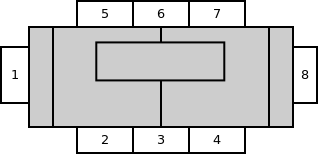
\includegraphics[width=3in]{pictures/mobot_connections}
	\end{center}
	\caption{Mobot Connection Locations.}
	\label{fig:mobot_connections}
\end{figure}
\begin{figure}[H]
	\begin{center}
		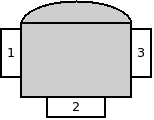
\includegraphics[width=2in]{pictures/linkbot_connections}
	\end{center}
	\caption{Linkbot Connection Locations.}
	\label{fig:linkbot_connections}
\end{figure}

\subsubsection{Accessories}
The accessories of the robots can be added to the scene and attached to the
robots by the tags.  Most accessories have multiple sides which are each
configured independently.  The options for a side are its id, robot which is
attached to that side, and the face of that robot.
\begin{verbatim}
<side id="1" robot="1" face="1"/>
\end{verbatim}

All sides are options which reside under the main accessory tag.  Each type of
robot has his own set of accessories.  Linkbot accessories are shown in Table
\ref{tab:linkacc} and Mindstorms accessories are shown in Table
\ref{tab:mindacc}.

\begin{table}[H]
	\begin{center}
	\begin{tabular}{c | c | c}
		\hline \hline
		\textbf{Number} & \textbf{Accessory} & \textbf{Num. of Sides} \\ \hline
		1 & BigWheel & 1 \\
		2 & Bridge & 2 \\
		3 & Caster & 1 \\
		4 & Cube & 5 \\
		5 & Faceplate & 1 \\
		6 & Gripper & 1 \\
		7 & Omniplate & 4 \\
		8 & Simple & 2 \\
		9 & SmallWheel & 1 \\
		10 & TinyWheel & 1 \\
		11 & Wheel & 1 \\
		\hline \hline
	\end{tabular}
	\caption{Linkbot Accessories}
	\label{tab:linkacc}
	\end{center}
\end{table}

\begin{table}[H]
	\begin{center}
	\begin{tabular}{c | c | c}
		\hline \hline
		\textbf{Number} & \textbf{Accessory} & \textbf{Num. of Sides} \\ \hline
		1 & Big Wheel & 1 \\
		2 & Small Wheel & 1 \\
		\hline \hline
	\end{tabular}
	\caption{Mindstorms Accessories}
	\label{tab:mindacc}
	\end{center}
\end{table}

\noindent
\newline
\textbf{Multiple Sided Accessories}
\newline
Accessories with multiple sides are configured with that number of
\verb%<side/>% tags as shown in this bridge example.
\begin{verbatim}
<bridge>
    <side id="1" robot="0" face="1"/>
    <side id="2" robot="1" face="3"/>
</bridge>
\end{verbatim}

This will connect a bridge between robots with ids 0 and 1 on the robot's faces
1 and 3, respectively.

\noindent
\newline
\textbf{One-Sided Accessories}
\newline
Accessories with only one side are configured with the robot and face options
within the robot tag as shown in the wheel example below.
\begin{verbatim}
<smallwheel robot="1" face="3"/>
\end{verbatim}

\noindent
\newline
\textbf{Daisy-Chaining}
\newline
Since accessories of the Linkbot can be attached to each other and not just
directly to the robot, there are options to daisy-chain the accessories
together.  To do this, the \verb%face% option is replaced for a side with the
\verb%conn% option and the number corresponding to the accessory shown in the
first column of Table \ref{tab:linkacc}.  The example below shows the simple
connector with a smallwheel attached to the third face of the robot.
\begin{verbatim}
<simple>
    <side id="1" robot="0" face="3"/>
    <side id="2" robot="0" conn="9"/>
</simple>
\end{verbatim}

\noindent
\newline
\textbf{Custom Wheel Sizes}
\newline
Custom wheel radii can be entered into the configuration file when using the
\verb%wheel% option.  The radii of the preconfigured big, small, and tiny wheels
are set internally to correspond to the produced wheels.  Inputting a custom
wheel radius is done through the \verb%side% option when daisy-chaining a wheel.
Below is a daisy-chained custom wheel with a radius of 0.001 meters.
\begin{verbatim}
<simple>
    <side id="1" robot="0" face="1"/>
    <side id="2" robot="0" conn="13" radius="0.001"/>
</simple>
\end{verbatim}

\subsection{Examples}
Some example configuration files.

\subsubsection{One Robot at (0, 0, 0)}
\begin{verbatim}
<?xml version="1.0" encoding="UTF-8"?>
<config>
    <version val="1"/>
    <type val="0"/>
	<grid units="1" major="12" tics="1" minx="-48" maxx="48" miny="-48" maxy="48"/>
    <tracking val="1"/>
</config>

<sim>
    <linkboti id="0">
        <position x="0" y="0" z="0"/>
        <rotation psi="0" theta="0" phi="0"/>
    </linkboti>
    <simple>
        <side id="1" robot="0" face="1"/>
        <side id="2" robot="0" conn="9"/>
    </simple>
    <simple>
        <side id="1" robot="0" face="3"/>
        <side id="2" robot="0" conn="9"/>
    </simple>
    <caster robot="0" face="2"/>
</sim>
\end{verbatim}

\subsubsection{Two Robots on X-Axis}
\begin{verbatim}
<?xml version="1.0" encoding="UTF-8"?>
<config>
    <version val="1"/>
    <type val="0"/>
	<grid units="1" major="12" tics="1" minx="-48" maxx="48" miny="-48" maxy="48"/>
    <tracking val="1"/>
</config>

<sim>
    <linkboti id="0">
        <position x="0" y="0" z="0"/>
        <rotation psi="0" theta="0" phi="0"/>
    </linkboti>
    <simple>
        <side id="1" robot="0" face="1"/>
        <side id="2" robot="0" conn="9"/>
    </simple>
    <simple>
        <side id="1" robot="0" face="3"/>
        <side id="2" robot="0" conn="9"/>
    </simple>
    <caster robot="0" face="2"/>
    <linkboti id="1">
        <position x="0.1524" y="0" z="0"/>
        <rotation psi="0" theta="0" phi="0"/>
    </linkboti>
    <simple>
        <side id="1" robot="1" face="1"/>
        <side id="2" robot="1" conn="9"/>
    </simple>
    <simple>
        <side id="1" robot="1" face="3"/>
        <side id="2" robot="1" conn="9"/>
    </simple>
    <caster robot="1" face="2"/>
</sim>
\end{verbatim}

\subsubsection{Explorer}
\begin{verbatim}
<?xml version="1.0" encoding="UTF-8"?>
<config>
    <version val="1"/>
    <type val="1"/>
	<grid units="1" major="12" tics="1" minx="-48" maxx="48" miny="-48" maxy="48"/>
    <tracking val="1"/>
</config>

<sim>
    <linkboti id="0">
        <position x="0" y="0" z="0"/>
        <rotation psi="0" theta="0" phi="-90"/>
    </linkboti>
    <linkboti id="1"/>
    <linkboti id="2" orientation="3">
        <joint f1="-20" f2="0" f3="20"/>
    </linkboti>
    <linkboti id="3">
        <joint f1="-90" f2="0" f3="90"/>
    </linkboti>
    <linkbotl id="4" orientation="3"/>
    <simple>
        <side id="1" robot="0" face="3"/>
        <side id="2" robot="0" conn="9"/>
    </simple>
    <simple>
        <side id="1" robot="1" face="1"/>
        <side id="2" robot="1" conn="9"/>
    </simple>
    <cube>
        <side id="1" robot="0" face="1"/>
        <side id="2" robot="0" conn="2"/>
        <side id="3" robot="1" face="3"/>
        <side id="5" robot="2" face="2"/>
    </cube>
    <bridge>
        <side id="1" robot="2" face="1"/>
        <side id="2" robot="3" face="1"/>
    </bridge>
    <bridge>
        <side id="1" robot="2" face="3"/>
        <side id="2" robot="3" face="3"/>
    </bridge>
    <simple>
        <side id="1" robot="3" face="2"/>
        <side id="2" robot="4" face="2"/>
    </simple>
    <gripper robot="4"/>
</sim>
\end{verbatim}

\newpage
\section{Appendix: Background Writing}
\label{app:backgrounds}
The RoboSim backgrounds which are available within the GUI are examples that can
be copied and modified to create custom background folders.  A full background
folder consists of the background XML file as well as the associated images to
be shown.

As an example the Outdoors background from the GUI is used here to show the
necessary items for a background.  Here is the list of files and folders within
the outdoors folder.
\begin{verbatim}
outdoors/sky/
outdoors/background.xml
outdoors/ground.3ds
outdoors/screenshot.png
\end{verbatim}

The sky folder holds all of the images which form the sky around the scene.
These are referenced in the \texttt{background.xml} file.  This file holds all
of the specifics for RoboSim to read and parse when loading your background.
The \texttt{ground.3ds} file is the green floor which is shown in the scene.
The screenshot is the image that is shown within the RoboSim GUI Backgrounds
list to show users what the background looks like.

The \texttt{background.xml} file is shown below:
\begin{verbatim}
<?RoboSim Background XML?>

<level>outdoors</level>

<name>Outdoors</name>

<screenshot>screenshot.png</screenshot>

<background>
    <ground>ground.3ds</ground>
    <front>sky/front.png</front>
    <left>sky/left.png</left>
    <back>sky/back.png</back>
    <right>sky/right.png</right>
    <top>sky/top.png</top>
    <bottom>sky/bottom.png</bottom>
</background>

<obstacles>
</obstacles>
\end{verbatim}

\subsection{Level}
The level is one of the default background options that can be extended with new
images.  The option goes within the \texttt{<level>} tags.  All of the options
are shown in Table \ref{tab:levels}.  \texttt{none} doesn't load any images and
only shows the black background.  \texttt{activitymat} is the small rectangle
mat from Barobo.  \texttt{board} loads a 4ft by 8ft board similar to the
RoboPlay Challenge Competition mats. \texttt{outdoors} is the large, expansive
environment.

\begin{table}[H]
	\begin{center}
	\begin{tabular}{c}
		\hline \hline
		\verb|none| \\
		\verb|activitymat| \\
		\verb|board| \\
		\verb|outdoors| \\
		\verb|RPC2017| \\
		\verb|RPC2016| \\
		\verb|RPC2015| \\
		\verb|RPC2014| \\
		\hline \hline
	\end{tabular}
	\caption{Levels}
	\label{tab:levels}
	\end{center}
\end{table}

\subsection{Name}
This is the name which will show up in the RoboSim GUI.  Pick something fun and
unique.

\subsection{Screenshot}
The name of your screenshot file.  The path to the file is relative to the xml
file location.  This image shows up in the background list to show off the cool
look of the background to others.

\subsection{Background}
All of the extra images to load for creating the environment are listed here.
The robots operate within a six-sided cube.  Each side, plus the ground, can
have an image.  If no image is provided, it will be left blank.

\subsection{Obstacles}
In addition to the required items shown above, an optional section which mimics
the RoboSim XML File (see Appendix \ref{app:xml}) is the obstacles tag.  Please
use the information from Section \ref{app:xml:obstacles} to add obstacles to the
background.  All obstacles added here are always loaded into the scene and
cannot be deleted by the RoboSim GUI.  All of the RoboPlay Challenge mats add
the border as a background obstacle so that it cannot be modified.

\end{document}

